\newpage
\subsection{Risikoanalyse}
Es gibt diverse Risiken, die während dieser Arbeit eintreten können. Um das Bewusstsein dafür zu stärken,
wird vorgängig eine Risikoanalyse durchgeführt, wobei es um die Identifikation wie auch die Zuordnung deren
Auftretenswahrscheinlichkeit und Auswirkungen geht. Weiterhin werden geeignete Massnahmen definiert, die entweder
die Eintrittswahrscheinlichkeit reduziert oder bei Auftreten angegangen werden können.

Die Risiken werden im Detail aufgelistet. Die Spalte \glqq WK\grqq{} steht für die Eintrittswahrscheinlichkeit, welche
in den Wahrscheinlichkeiten \glqq Gering\grqq, \glqq Möglich\grqq, \glqq Wahrscheinlich\grqq, \glqq Sehr Wahrscheinlich\grqq{}
angegeben wird. Die Spalte \glqq AW\grqq{} steht für die Auswirkungen, welche in den Grössen \glqq Klein\grqq, \glqq Mittel\grqq, \glqq Gross\grqq{}
angegeben wird.

\begin{table}[ht]
    \rowcolors{1}{\seccolor!10}{\seccolor!10} % Rows with 10% of secondary color
    \begin{tabularx}{\linewidth}{llXll}
        \rowcolor{\seccolor!50}
        ID & Risiko & Massnahme & WK & AW\\\bfhmidline

        R-1 & Verlust von Programm-Sourcen & Führen eines Repositories auf GIT, welches das Wiederherstellen
        eines bestimmten Standes erlaubt. Jeder Entwickler hat durch GIT eine lokale Kopie der Sourcen. Zudem wird jeden Freitag
        ein Backup des GIT-Standes auf eine externe Festplatte
        geschrieben, sollte der unwahrscheinliche Fall eintreten, dass
        GIT nicht mehr verfügbar sein sollte oder seine Bestände verliert. & Gering & Gross\\\bfhmidline

        R-2 & Ausfall der Arbeitsgeräte & Es stehen Ersatzgeräte bereit, welche sofort zum Einsatz
        kommen könnten. & Möglich & Klein\\\bfhmidline

        R-3 & Krankheitsausfall der Teammitglieder & Es wird, wenn möglich von Zuhause aus gearbeitet,
        um das Risiko einer Ansteckung zu vermindern. & Möglich & Gross\\\bfhmidline

        R-4 & Parallele Entwicklung derselben Funktionen & Durch eine anfängliche Planung der Arbeitspakete, wie
        auch den ständigen Austausch und Einsatz von
        Pair-Programming an geeigneten Stellen, wird
        das Risiko stark reduziert. Sollte es trotzdem
        Eintreten, sind die Auswirkungen marginal, da die
        ständige Kommunikation dies sofort aufdecken würde. & Gering & Klein\\\bfhmidline

        R-5 & Unterschätzen der Komplexität & Um zumindest ein brauchbares Resultat vorweisen zu können,
        wurde der erste Meilenstein möglichst simpel gehalten. & Wahrscheinlich & Gross\\\bfhmidline

        R-6 & Verpassen wichtiger Termine & Es wird ein Kalender mit allen Terminen geführt, welcher mehrmals eine
        Erinnerung anzeigt.& Gering & Gross\\\bfhmidline
    \end{tabularx}
    \caption{Risiken}
    \label{tab:risiken}
\end{table}

Die identifizierten Risiken werden in der Abbildung \ref{fig:risikoanalyse} für eine bessere Übersicht eingetragen.
\begin{figure}[h!]
    \begin{center}
        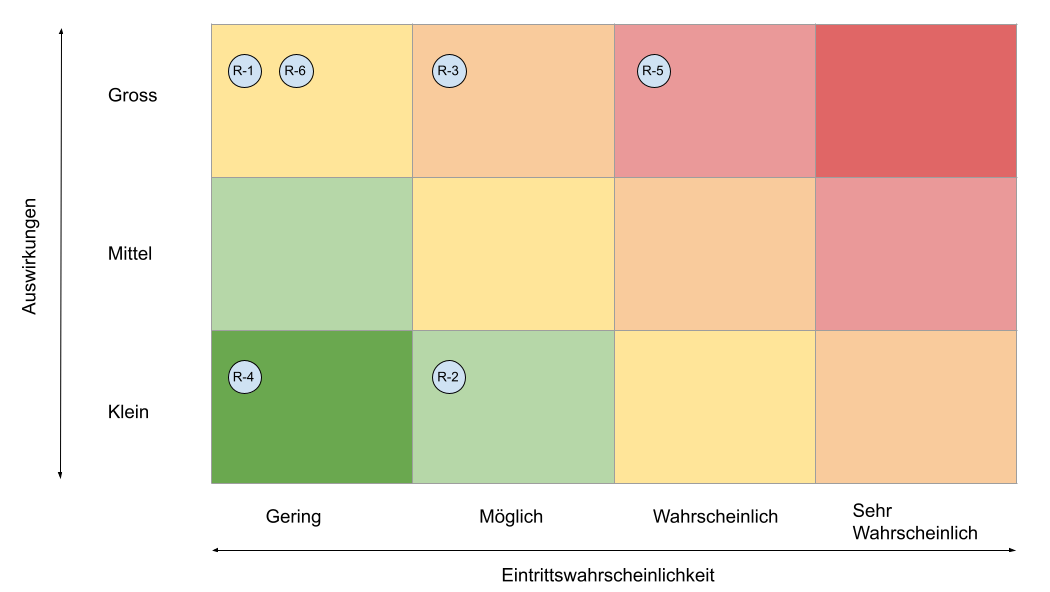
\includegraphics[width=0.8\linewidth]{../common/03_billiard_ai/resources/16_risikoanalyse.png}
    \end{center}
    \caption{Risikoanalyse}
    \label{fig:risikoanalyse}
\end{figure}